% Shared preamble for the English summaries in this repository.
\documentclass[11pt,a4paper]{article}
\usepackage[margin=2.2cm]{geometry}
\usepackage[T1]{fontenc}
\usepackage[utf8]{inputenc}
\usepackage{lmodern}
\usepackage{amsmath,amssymb}
\usepackage{graphicx}
\usepackage{booktabs}
\usepackage{enumitem}
\usepackage[hidelinks]{hyperref}
\setlist{itemsep=2pt,topsep=4pt}
\setlength{\parindent}{0pt}
\setlength{\parskip}{5pt}
\graphicspath{{figures/}}
\newcommand{\summaryheader}[3]{%
  \begin{center}
    {\Large\bfseries #2}\\[3pt]
    {\large #1}\\[3pt]
    {\small Arshia Goshtasbi \textbullet{} MSc Electrical Engineering (Control), Iran University of Science and Technology \textbullet{} #3}
  \end{center}
  \vspace{2pt}\hrule\vspace{8pt}
  \noindent\textit{English summary of my original Persian report, which is kept as a PDF in this folder.}\par}

\begin{document}
\summaryheader{Optimal Control, Homework 4}{Finite-horizon LQR in Simulink (Kirk Examples 5.2-1 and 5.2-2)}{Spring 1404 (2025)}

\section*{Example 5.2-1: first-order plant (\texttt{Q5\_2\_1.slx})}
I simulated the finite-horizon LQR for a first-order plant with $a=0.2$ (unstable) and $a=-0.2$ (stable), and plotted the Riccati gain $k(t)$, the control $u(t)$ and the state $x(t)$. With $a=0.2$ the control is larger, because the controller has to work against the instability. Each case was run for several values of the terminal weight $H$. A larger $H$ makes the control a little larger, because the controller works harder to shrink the final error that $J$ penalises.

\section*{Example 5.2-2: second-order plant (\texttt{Q5\_2\_2.slx})}
The method in the course is offline: the Riccati differential equation is integrated backwards from $t_f=15$\,s before the simulation. \texttt{Q5\_2\_2\_Gains.m} does this with \texttt{ode45} for $K_{11}$, $K_{12}$ and $K_{22}$ and stores them as time series. The Simulink model then applies $u(t)=-R^{-1}B^TK(t)x(t)$ to the double-integrator-type plant.

\begin{center}
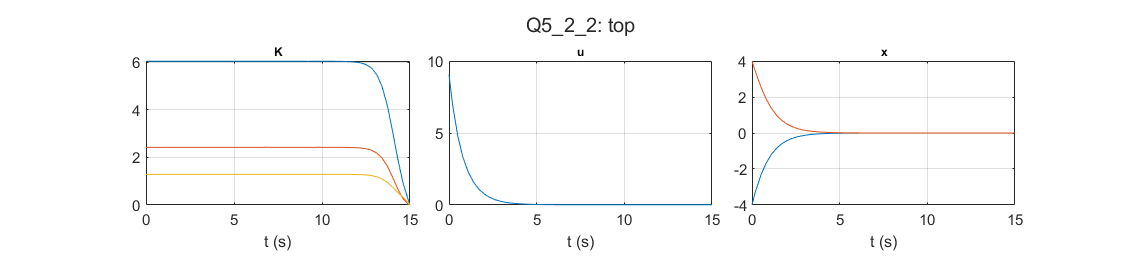
\includegraphics[width=0.75\linewidth]{Q5_2_2_scopes.png}\\[2pt]
{\small Re-run in R2023b: Riccati gains $K(t)$, control $u(t)$ and states $x(t)$.}
\end{center}
\begin{center}
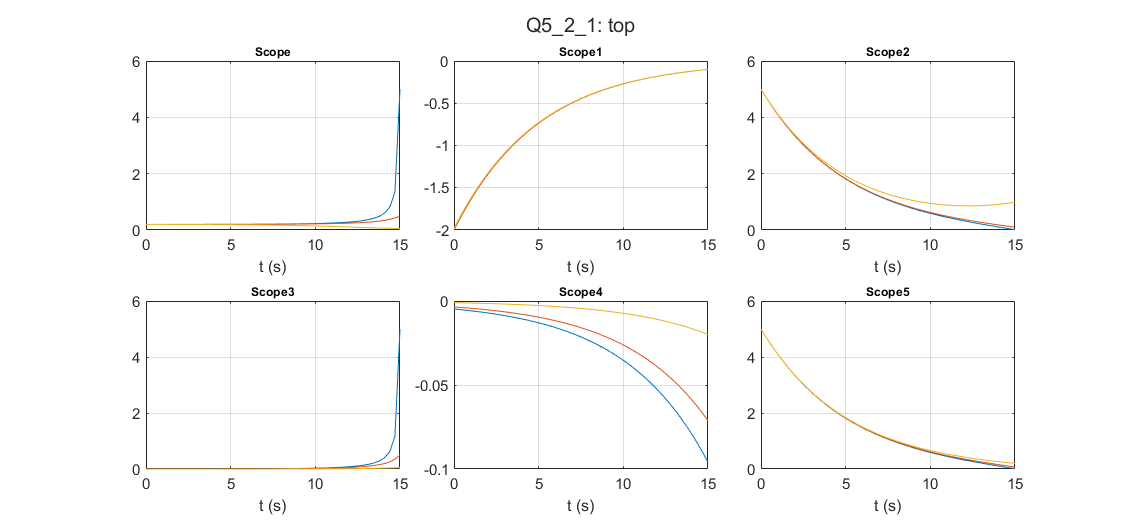
\includegraphics[width=0.62\linewidth]{Q5_2_1_scopes.png}\\[2pt]
{\small Example 5.2-1: scopes of the six sub-models.}
\end{center}

\textit{How to run:} run \texttt{Q5\_2\_2\_Gains.m} first, then \texttt{Q5\_2\_2.slx}.
\end{document}
